% WORKING DRAFT v2 of the MARL paper.  Revision 30/09/2026 19:xx EDT (ledger L-178): novelty framing after a collision
% review, the corrected V-U (same-information null), the zero-byte bar's own seed variance, the negative deadline-head
% test, figures from saved reports, and a verified bibliography.  The 16:0x version is kept at
% legacy/source_backups/paper_marl_v2_pre_novelty_20260930_1859.tex; paper_marl.tex (v1) is kept unchanged.
% Part I (analysis + minimal fix) rests on evidence in hand.  Part II (direct checks of mechanism predictions) is
% measured; its E3-specific statements are NOT in Lean (rule: nothing enters as a theorem before compiled, gated Lean),
% so they appear as claims with proof sketches.  Every number is copied from a named ledger row of
% research/papers/audits/MARL_SELF_AUDIT_LEDGER_20260928.md (tags L-xxx in the notes) and its artifacts.
% All E3 results are DEVELOPMENT or DEVELOPMENT-CONFIRM (pre-registered, unused panels); the reserved test 1301-1316 is closed.
% Figures: scripts/MARL_make_figs_v2.py (reads saved report JSONs only) -> figs_v2/*.pdf, numbers in figs_v2/figures_data.json.
% Build: tectonic -X compile paper_marl_v2.tex --keep-logs
\documentclass[11pt]{article}
\usepackage[margin=1in]{geometry}
\usepackage{amsmath,amssymb,amsfonts,amsthm}
\usepackage{graphicx,booktabs,url,xcolor}
\usepackage{tikz}
\usetikzlibrary{positioning,arrows.meta,calc}
\usepackage[hidelinks]{hyperref}
\graphicspath{{figs_v2/}}

\newtheorem{claim}{Claim}
\theoremstyle{definition}
\newtheorem{definition}{Definition}
\newtheorem{prediction}{Prediction}

\newcommand{\lean}[1]{\textsf{\footnotesize #1}}
\newcommand{\PROVED}{\textsc{proved}}
\newcommand{\NUM}{\textsc{numerical}}
\newif\ifshownotes\shownotestrue
\definecolor{notecol}{RGB}{0,70,190}
\definecolor{todocol}{RGB}{190,20,20}
\newcommand{\NOTE}[1]{\ifshownotes{\color{notecol}\,\textsf{\footnotesize[N: #1]}}\fi}
\newcommand{\TODO}[1]{\ifshownotes{\color{todocol}\,\textsf{\footnotesize[TODO: #1]}}\fi}
\newcommand{\TODOPAR}[1]{\ifshownotes\par\vspace{2pt}\noindent%
  {\color{todocol}\textsf{\footnotesize\textbf{To decide.}\;#1}}\par\vspace{2pt}\fi}

\begin{document}
\sloppy
% Previous title (16:0x): "Silence Is a Strong Baseline: Relay, Rotation and the Distilled Zero-Byte Bar for
% Prefix-Broadcast Multi-Agent Communication".  Changed because its framing is close to Chauhan and Bera (2026).
\title{Relay Needs Rotation: Fresh Decision Coverage and a Compiled-Silence Bar\\
for Prefix-Broadcast Multi-Agent Communication}
\author{\TODO{authors and affiliation}}
\date{Working draft v2, 30 September 2026}
\maketitle

\TODOPAR{(1) Venue and page limit are unconfirmed; they decide how much of Part II moves to an appendix.
(2) Title: authors decide; the previous title (``Silence is a strong baseline'') is close in framing to~\cite{chauhan2026}.
(3) Reserved test (traffic seeds 1301--1316), once, after a design freeze. (4) More training seeds (at least five
teacher/student pairs) and a second road network: heavy runs, planned on another machine. (5) Lean for Claims~1--3 is
paused by the authors.}

\begin{abstract}
We study learned communication when several agents share one committed broadcast stream and each receiver decodes only
a prefix of it, of a size that varies between receivers and over time. On a $3\times3$ CityFlow traffic-signal grid
with such a channel, we evaluate communication against a stronger comparator than a separately trained silent agent: a
\emph{compiled-silence} student, distilled from a full-information teacher, that sends zero bytes. Controls show that
its gain is the teacher's information, not distillation or compute. Against this bar, every design inside the packet
channel that we pre-registered fails or is seed-dependent. We trace the failures to three interacting mechanisms of
prefix decoding: sparse sender exposure in a slot-indexed input, stale cached copies, and a congestion-ranked stream
head that starves low-ranked senders. The established tools do not suffice on their own: relay tables plus
distillation reach every sender but, under the natural head order, carry stale copies and lose to compiled silence at
low capacity on a pre-registered panel. Adding an age-first stream order, which rotates which senders are transmitted, inside the same 25-byte packets and byte accounting,
beats the bar on that panel in all six cells (two seeds, three capacity conditions; $-2.2$ to $-4.0\%$ total waiting),
and against a second, stronger zero-byte student on development data. Direct probes connect the repair along a chain:
age-first rotation keeps every sender injected, and relay turns that into short ages at every receiver; age and decision margin govern agreement with the fresh-information action; relay
recovers the teacher's decision on 19--34 points more of the steps where a zero-byte student errs than a second
zero-byte student does; and teacher agreement tracks closed-loop waiting across twelve conditions ($r=-0.93$). The
operative resource is fresh, decision-relevant coverage, not packet count.
\end{abstract}

\part*{Part I --- Analysis and a minimal fix}

\section{Introduction}\label{sec:intro}
\begin{figure}[t]
\centering
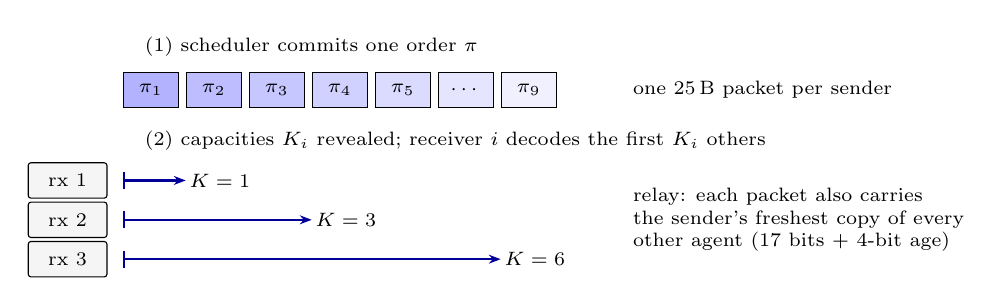
\begin{tikzpicture}[font=\scriptsize, pkt/.style={draw, minimum width=7mm, minimum height=4.5mm, inner sep=0pt},
  rx/.style={draw, rounded corners=1pt, minimum width=10mm, minimum height=4.5mm, fill=black!4}]
\node[anchor=west] at (-0.2,1.05) {(1) scheduler commits one order $\pi$};
\foreach \i/\lab in {0/$\pi_1$,1/$\pi_2$,2/$\pi_3$,3/$\pi_4$,4/$\pi_5$,5/$\cdots$,6/$\pi_9$}
  \node[pkt, fill=blue!\the\numexpr 30-4*\i\relax] (p\i) at (\i*0.8,0.5) {\lab};
\node[anchor=west] at (6.0,0.5) {one 25\,B packet per sender};
\node[anchor=west] at (-0.2,-0.15) {(2) capacities $K_i$ revealed; receiver $i$ decodes the first $K_i$ others};
\foreach \r/\k/\y in {1/1/-0.65,2/3/-1.15,3/6/-1.65}{
  \node[rx, anchor=east] (r\r) at (-0.55,\y) {rx $\r$};
  \draw[|-{Stealth[length=1.5mm]}, thick, blue!60!black] ($(p0.west)+(0,\y-0.5)$) -- ++(\k*0.8,0) node[right, inner sep=1pt, black] {$K=\k$};
}
\node[anchor=west, align=left] at (6.0,-1.15) {relay: each packet also carries\\ the sender's freshest copy of every\\ other agent (17 bits + 4-bit age)};
\end{tikzpicture}
\caption{The prefix-broadcast channel (PROTOCOL\_HETERO\_v0). A receiver with a small capacity hears only the head.
With the default congestion-ranked order the same senders stay at the head, so low-ranked senders are rarely injected
(starvation); relay spreads their last copies, which then age.}
\label{fig:channel}
\end{figure}

Budgeted multi-agent communication is usually evaluated against agents trained without messages. We study a channel,
and a comparator, where that evaluation is too weak. One broadcast stream is committed per step. After it is committed,
each receiver learns how many packets it can decode, and it decodes the first $K_i$ of the stream
(Figure~\ref{fig:channel}). Capacities differ between receivers and change every step. Layered and priority-encoded
multicast to heterogeneous receivers is classical in networking~\cite{rlm,pet}. We are not aware of prior MARL
evaluations under this specific receiver-dependent prefix-decoding constraint.

\paragraph{Findings.}
\begin{enumerate}
\item \textbf{Compiled silence is the right bar.} A zero-byte student distilled from a full-information teacher beats a
co-trained silent actor on five of five seeds. Controls show the gain is the teacher's information
(Section~\ref{sec:student}). Learned actors that use the channel's own deliveries lose even to the weaker silent actor.
Communication is known to lose to silence in other settings~\cite{chauhan2026,caic}; what we add is the stronger,
compiled comparator and the anatomy of the loss in this channel.
\item \textbf{Three interacting mechanisms} (Section~\ref{sec:mech}): sparse sender exposure in a slot-indexed input,
stale cached copies, and head starvation at low capacity.
\item \textbf{Established tools are not enough on their own.} Relay tables with distillation reach every sender, but
under the natural head order they carry old copies. On a pre-registered panel they lose to compiled silence at low
capacity for one of two seeds, and against a second zero-byte student they fail or tie in all four low-capacity cells
(Section~\ref{sec:fix}).
\item \textbf{Coverage plus freshness repairs it.} An age-first stream order, inside the same packets and byte accounting,
turns relay's coverage into fresh coverage and beats the bar in all six pre-registered cells.
\item \textbf{A measured chain} (Part II): age-first rotation keeps every sender injected and relay keeps ages short; age and margin govern decision agreement; on the steps where the zero-byte student errs, relay recovers the teacher's decision far more often than a
same-information null does; and decision agreement tracks waiting.
\end{enumerate}

\paragraph{Contributions, scoped.}
We do \emph{not} introduce relay, distillation, compression or freshness scheduling; each is established
(Section~\ref{sec:related}). We contribute:
\begin{itemize}
\item (i) this channel as a MARL stress test, with explicit byte accounting and an oracle-access audit;
\item (ii) compiled silence as an audit principle for deployment-time communication claims, with controls for
distillation, compute, dose and the bar's own seed variance;
\item (iii) a failure anatomy with every alternative hypothesis tested by a rule written before its result;
\item (iv) the demonstration, pre-registered, that relay alone fixes coverage but not freshness and that a fair head
completes the repair under the unchanged byte contract;
\item (v) direct probes of each link of the mechanism chain, including a same-information null and a negative
targeted-refresh test.
\end{itemize}

\section{Related work}\label{sec:related}
\paragraph{Silence and failure of learned communication.} Chauhan and Bera~\cite{chauhan2026} find, at matched 2-bit
rates over 25 seeds, that learned senders are often indistinguishable from silence while engineered senders succeed.
They localise the failure in protocol discovery. Our failure is of a different kind: engineered, structured payloads
lose because of how a prefix channel exposes, ages and orders them. CAIC~\cite{caic} models a shared channel as a
queue and finds stale messages under delay can be worse than none. I2C~\cite{i2c} notes that broadcast redundancy can
impair learning.
\paragraph{Learned communication under budgets.} SchedNet~\cite{schednet} learns who broadcasts, and
IMAC~\cite{imac} learns messages and schedules jointly. NDQ~\cite{ndq}, information-bottleneck and vector-quantised
messages~\cite{ibvq}, event-triggered sending~\cite{etcnet} and Where2comm~\cite{where2comm} reduce bytes.
CACOM~\cite{cacom} personalises messages per receiver after a coarse broadcast. We instead keep one common ordered
broadcast that receivers decode to different depths, and ask what can be recovered under that constraint.
\paragraph{Multi-hop, global and delayed information.} Multi-hop and global dissemination are well studied:
\begin{itemize}
\item imitation of centralised experts by graph controllers with delayed $k$-hop information~\cite{gama2022,tolstaya2019};
\item recurrent delayed global messages in traffic control (NeurComm~\cite{neurcomm});
\item message chains (TEM~\cite{tem}), two-hop relays (AC2C~\cite{ac2c}), full-team recurrent chains
(FCMNet~\cite{fcmnet}) and low-diameter topologies with memory (ExpoComm~\cite{expocomm});
\item protocols that make every agent reconstruct the state uniformly (LMAC~\cite{lmac}).
\end{itemize}
Delay-aware communication is also established: DACOM~\cite{dacom}, CoDe~\cite{code}, the value-of-information
prioritisation of VIL2C~\cite{vil2c}, and the gain/delay-cost decomposition of CGDC~\cite{cgdc}. Our relay tables are
an instance of this family. What we add is the observation that, under prefix decoding, relay alone yields
\emph{stale} global coverage, and the head order decides whether that coverage is fresh.
\paragraph{Freshness and scheduling.} Keeping every source fresh on a shared channel is age-of-information scheduling.
In symmetric broadcast networks the greedy highest-age-first policy, which our age-first head instantiates, is
optimal~\cite{kadota2018}, and round-robin is $O(1)$-competitive under packet management~\cite{jien2023}. Freshest-copy
merging of timestamped relays is gossip; its age scales with network size as analysed in~\cite{yates2021,selen2013}.
Periodic per-source deadlines are pinwheel scheduling; every instance of density at most $5/6$ is
schedulable~\cite{kawamura2024}. One broadcast for clients with different needs is broadcast disks~\cite{broadcastdisks}.
One order serving every cardinality is incremental maximisation~\cite{bernstein2022,bienkowski2026}. Embedding
priorities so that any prefix decodes the important part is Priority Encoding Transmission~\cite{pet}. One sequence
serving every house size within quota is house-monotone apportionment~\cite{balinski1982}.
\paragraph{Privileged teachers and communication-free students.} Distilling centralised or privileged teachers into
decentralised students is established:
\begin{itemize}
\item CTDS~\cite{ctds}, PTDE~\cite{ptde}, HINT~\cite{hint}, communication-enhanced tutoring~\cite{tutoring},
KD-MARL~\cite{kdmarl} and MAGPO~\cite{magpo};
\item communication-free students specifically: CoDiMAD~\cite{codimad}.
\end{itemize}
These works ask whether privileged training improves decentralised execution. We ask a different question: does
runtime communication add value beyond the coordination that can already be compiled into a zero-byte policy? We
therefore use the student as a comparator and as a training route, not as a contribution.
\paragraph{Traffic.} CityFlow~\cite{cityflow}; CoLight~\cite{colight}; UniComm~\cite{unicomm}, which already sends
compact predictions of neighbour impact; max pressure~\cite{varaiya2013}; MAPPO~\cite{mappo}; DAgger~\cite{dagger}.

\section{Setting}\label{sec:setting}
\paragraph{Channel (PROTOCOL\_HETERO\_v0).} The $m=9$ intersections are senders and receivers. At each of 26 decision
steps (10\,s apart) the scheduler commits an order $\pi$ of the senders. Receiver capacities $K_i$ are then revealed,
and receiver $i$ decodes $S_i$, the first $K_i$ senders of $\pi$ other than itself. We use three capacity conditions:
\begin{itemize}
\item iid: $K_i\sim U\{1,\dots,7\}$ per receiver and step;
\item \emph{cap4}: the stream capped at 4 packets;
\item \emph{low}: $K_i\sim U\{1,2,3\}$.
\end{itemize}
A frontier study uses a constant $K$. Packets are 25\,B, and a profile is charged for its stream prefix plus its
description, exactly as in the protocol. The average step costs 188.7\,B under iid, 100\,B under cap4 and about 94\,B
under low. A receiver keeps its last direct copy of every sender. Transport delay is zero: every age in this paper comes
from which packets are decoded, not from latency.
\paragraph{Information.} The scheduler may use:
\begin{itemize}
\item the payloads paid in earlier steps and their measurement times;
\item a mirror of every receiver's cache;
\item the public topology and the actor code.
\end{itemize}
Fresh states, counterfactual views and oracle rollouts are used only as training labels or labelled diagnostics. Every
evaluation runs a per-step access audit, and every oracle call inside a deployable path raises.
\paragraph{Task.} CityFlow $3\times3$ grid, headways 8 and 16\,s. The metric is total queue (waiting) per episode.
\begin{itemize}
\item Development panel: traffic seeds 901--964 $\times$ both headways (128 episodes).
\item Pre-registered panels use unused seed blocks between 2001 and 2664, each used once.
\end{itemize}
Comparisons are paired by episode and reported as the ratio of summed waiting minus one, with 95\% bootstrap intervals
over traffic seeds (both headways resampled together, 4000 draws).

\section{Actors, training and comparators}\label{sec:methods}
\paragraph{Actors.} A flat actor concatenates eight sender blocks (fresh flag, heard flag, age, phase, elapsed,
vehicles and waiting per approach, static topology) with the receiver's own state into an MLP. A \emph{set} actor applies
one shared encoder to each present sender block and mean-pools over present senders, so absent senders contribute
nothing. Both are trained by MAPPO with a centralised critic~\cite{mappo}.
\paragraph{Teacher and students.} The \emph{teacher} is a set actor trained with full, fresh delivery (every receiver
decodes all 8 senders every step). A \emph{student} is trained by DAgger~\cite{dagger}: it acts on its own deployment
input, the teacher labels its states from the counterfactual full view (a training-only oracle), and the teacher mixture
$\beta$ decays from 1 to 0 over the first half of 500 iterations.
\paragraph{Comparators.}
\begin{itemize}
\item \emph{maxq}: serve the approach with the largest queue; 0 bytes.
\item \emph{set\_none}: a set actor co-trained with no messages.
\item \emph{Compiled silence (the zero-byte student)}: the teacher distilled into a policy with no message input. A
second one per teacher, identical except its seed, measures the bar's own variance.
\item \emph{FO}: the teacher deployed with a fresh-only receiver, which drops stale cached blocks.
\item \emph{BYTEBUDGET}, a reference in a different channel model: receiver byte capacity $25K_i$, with 3\,B packets, so
that every receiver decodes all 8 senders at 27\,B per step.
\end{itemize}
\paragraph{Relay packets.} Sender $k$'s 25\,B packet carries positional slots:
\begin{itemize}
\item its own 17-bit summary: phase 4, elapsed 1, vehicles $2\times4$, waiting $1\times4$ bits;
\item for each other agent $j$, the same 17 bits of the freshest summary of $j$ that $k$ holds, plus a 4-bit age in
decision steps, saturated at 14, with 15 meaning absent.
\end{itemize}
That is $17+8\times21=185$ bits $\le 200$. The table grows linearly in $m$, so this layout fits a 25\,B packet only for
small teams (Section~\ref{sec:limits}). Summary levels come from a codebook fitted on training traffic. A receiver
merges the packets it decodes with its own cache, keeping the freshest copy per agent.
\NOTE{L-162, L-165 (the byte-layout audit), L-174 (the saturated-age re-measure).}
\paragraph{Stream order.}
\begin{itemize}
\item \emph{Default}: the scheduler's cached-queue ranking.
\item \emph{Age-first} (``rotation''): senders whose last transmitted packet is oldest go first. What rotates is the
set of transmitted senders, not necessarily the head (Claim~\ref{cl:age}).
\end{itemize}
Both use scheduler information only. The cap rule is applied under every order.\NOTE{L-168: a tooling bug that
ignored cap4 under agefirst was found and fixed before any affected run.}

\section{Failures: messages harm, and why}\label{sec:fail}
\paragraph{Learned actors that use their messages are worse than silence.} On the development panel, a flat actor
trained with the same recipe but no messages has $8.0\%$ $[7.4,8.6]$ less waiting than the committed-prefix system of
five flat prefix-trained actors, and less than each of them ($5.6$ to $10.5\%$). A second training seed gives $7.9\%$.
Doubling the prefix actor's training to 4000 iterations leaves it $6.3\%$ $[5.3,7.4]$ worse than the silent actor at
equal iterations.\NOTE{L-105, L-109, L-113.}
\paragraph{The heuristic reference was harmed by its own messages.} Max pressure as implemented has about 14\% MORE
waiting than the same rule without its downstream (message-fed) terms. That max-queue rule uses no messages, and every
pressure variant tried is worse still. Against max-queue, warm-started actors cloned from max pressure are worse
($+1.2$ to $+5.5\%$), and flat prefix actors are only $1.7$--$6.3\%$ better.\NOTE{L-114--L-116.}
\paragraph{Selecting messages does not fix it.} An earlier line of work scheduled messages for frozen prefix-trained
actors. No legal selector beat the committed prefix in closed loop (Appendix~\ref{app:history}). The oracle headroom
behind that effort is, to first order, best-of-N over action perturbations of an imperfect actor: forcing one agent's
action with no message change reaches the same oracle.\NOTE{L-78, L-81.}

\section{Mechanisms of the failure}\label{sec:mech}
We wrote each hypothesis and its reading rule before its result.
\paragraph{Sparse, varying sender sets in a slot-indexed input.}
\begin{itemize}
\item A flat actor trained with full delivery keeps 79--85\% of its full-information gain when 5--7 of 8 senders are
present.
\item It falls below the silent actor under the protocol's capacity process, where about half the senders are absent:
$+4.2$ and $+1.3\%$ on two seeds.
\item Mean pooling over present senders (the set actor) degrades gracefully; attention pooling equals mean pooling.
\item Three alternatives are refuted by their rules: irrelevant input dimensions (H1), stale content alone (H5), and
weight sharing without pooling (H3). Doubling the width (H7) does not close the gap.
\item Under 25\% packet loss the set receiver keeps its advantage, and the flat one breaks.
\end{itemize}
\NOTE{L-132, L-133, L-135, L-142, L-157.}
\paragraph{Stale cached copies.}
\begin{itemize}
\item The full-information set teacher, deployed under the prefix with its stale cached blocks, is no better than
set\_none: $-0.1\%$ $[-1.0,+0.9]$.
\item Dropping stale blocks at the receiver (FO) recovers 59\% of the full-information gain: $-3.3\%$ on the development
panel, $-3.0\%$ and $-5.2\%$ for two seeds on a pre-registered panel.
\end{itemize}
\NOTE{L-124, L-125, L-127, L-138.}
\paragraph{Head starvation at low capacity.}
\begin{itemize}
\item The default order ranks senders by cached congestion. When few packets are decoded, the same senders stay at the
head.
\item In a traffic-free replica of the channel, validated against measured ages, a sticky ranking at cap4 leaves 40--46\%
of (receiver, agent) pairs never covered.
\item With relay packets in CityFlow the pairs are still covered, but copies are old: the mean relayed age is 5.4 decision
steps, and 45\% of copies are at least 4 steps old, under cap4 and low.
\item Age-first rotation gives ages of 0.8--1.4 steps, with 0--5\% of copies at least 4 steps old.
\end{itemize}
\NOTE{L-168 (simulator), L-177 (probe ages).}

\section{The bar: compiled silence}\label{sec:student}
\paragraph{Gain.} Development panel, five training seeds: the zero-byte student has $3.5\%$ $[2.2,4.9]$ less waiting than
set\_none, and less on every seed.\NOTE{L-160; two-level bootstrap over training and traffic seeds.}
\paragraph{Controls.}
\begin{itemize}
\item \emph{Distillation alone:} the same DAgger recipe with a silent teacher gives $+0.2$, $-0.2$ and $+0.2\%$ against
set\_none on three seeds.
\item \emph{Extra compute:} 500 more PPO iterations for set\_none give $+2.0\%$.
\item \emph{Dose:} the gain grows with the teacher's information. Against set\_none, a silent teacher gives $\approx0$, a
prefix-message teacher $-2.3/-0.9\%$, and a full-information teacher $-3.2/-6.3\%$ (two seeds).
\end{itemize}
The gain is therefore communication used at training time and compiled into a local policy.\NOTE{L-147, L-149, L-152,
L-153, L-158.}
\paragraph{The bar has its own seed variance.} A second zero-byte student per teacher, trained identically except for its
seed, differs from the first by $-0.26\%$ $[-1.08,+0.55]$ (seed 0) and $-1.20\%$ $[-1.99,-0.49]$ (seed 1). A single
student per teacher can therefore understate the bar by about one percent, and claims should be checked against more
than one.\NOTE{L-178; eval v6 as for the first student.}
\paragraph{Designs inside the packet channel measured against the bar} (pre-registered, unused panels, both seeds
required):
\begin{center}\small
\begin{tabular}{@{}lccl@{}}
\toprule
design & seed 0 & seed 1 & verdict\\
\midrule
FO vs set\_none & $-3.0\%$ & $-5.2\%$ & passes against the weak bar\\
FO vs the zero-byte student & $+1.3\%$ & $+2.1\%$ & the student is better\\
fresh-only student vs the zero-byte student & $-0.8\%$ (fail) & $-4.0\%$ & seed-dependent\\
set\_fresh vs the zero-byte student & $-2.0\%$ & $+7.2\%$ (fail) & seed-dependent\\
\bottomrule
\end{tabular}
\end{center}
Extra seeds confirm the reading: set\_fresh is typically about $-2\%$ against set\_none and does not beat the student.
\NOTE{L-127, L-129, L-138, L-140, L-141, L-144--L-146, L-150.}

\section{The fix: coverage by relay, freshness by rotation}\label{sec:fix}
\paragraph{Relay removes sparse exposure inside the packet channel.} On the development panel, the relay student under
the default order beats the zero-byte student by $3.3\%$ $[2.5,4.2]$ and $4.0\%$ $[3.1,5.0]$ (iid), with the channel and
its accounting unchanged. That ties the byte-budget reference. With no messages it is $4.8\%$ worse than the student, so
it uses them.\NOTE{L-163; unchanged under saturated ages, L-174.}
\paragraph{Relay alone is not enough.} Under the default order relay loses its advantage at low capacity. Seed 0 is
$+0.9\%$ (cap4) and $+0.4\%$ (low) against the student on the development panel. Against the second zero-byte student,
relay under the default order is:
\begin{itemize}
\item seed 0: $+1.21\%$ $[+0.28,+2.20]$ at cap4 and $+0.61\%$ $[-0.14,+1.40]$ at low;
\item seed 1: $-0.42\%$ $[-1.22,+0.44]$ at cap4 and $-0.20\%$ $[-1.08,+0.72]$ at low.
\end{itemize}
Relay plus distillation, the combination of established tools, thus fails or ties in all four low-capacity cells.
\NOTE{L-169, L-174, L-178.}
\paragraph{Rotation makes the coverage fresh.} Age-first rotation restores the advantage on the development panel:
\begin{itemize}
\item cap4: $-2.3$ / $-4.1\%$ (seed 0 / seed 1);
\item low: $-2.8$ / $-3.0\%$;
\item the iid cost of rotation is small and not significant on these panels: $+0.3$ / $+0.9\%$.
\end{itemize}
Against the second, stronger zero-byte student it still wins in all six cells: $-2.80$, $-2.01$, $-2.55\%$ (seed 0; iid,
cap4, low) and $-1.99$, $-2.98$, $-1.78\%$ (seed 1), every upper bound below zero.\NOTE{L-169, L-174, L-178.}

\begin{figure}[t]
\centering
\includegraphics[width=0.62\linewidth]{fig_prereg.pdf}
\caption{Pre-registered panel 2601--2664 (128 episodes, used once): total waiting against the same-seed zero-byte
student, 95\% bootstrap over traffic seeds. Filled: the primary endpoint (relay with age-first rotation); every upper bound
is below zero. Hollow: relay under the default order (secondary), which loses at low capacity for seed 0.
\NOTE{scripts/MARL\_make\_figs\_v2.py from e3\_relayrot\_panel\_report\_20260930.json; L-175.}}
\label{fig:prereg}
\end{figure}

\paragraph{Pre-registered confirmation.} We registered the protocol before any run, on panel 2601--2664 (checked unused).
The primary endpoint is relay with age-first rotation against the same-seed zero-byte student. All six cells (two seeds
$\times$ three capacity conditions) had to have an upper 95\% bound below zero.
\begin{center}\small
\begin{tabular}{@{}lccc@{}}
\toprule
& iid (189\,B/step) & cap4 (100\,B/step) & low ($\approx94$\,B/step)\\
\midrule
seed 0 & $-2.19\%$ $[-3.10,-1.25]$ & $-2.96\%$ $[-3.87,-2.04]$ & $-2.19\%$ $[-2.95,-1.43]$\\
seed 1 & $-4.00\%$ $[-4.71,-3.30]$ & $-3.41\%$ $[-4.09,-2.75]$ & $-2.43\%$ $[-3.20,-1.67]$\\
\midrule
\multicolumn{4}{@{}l}{\emph{secondary, same panel}}\\
relay, default order, seed 0 & $-2.71\%$ & $+0.68\%$ $[-0.12,+1.50]$ & $+0.96\%$ $[+0.10,+1.88]$\\
relay, default order, seed 1 & $-4.29\%$ & $-1.76\%$ & $-1.74\%$\\
\bottomrule
\end{tabular}
\end{center}
The primary endpoint is supported in all six cells (Figure~\ref{fig:prereg}). The same panel reproduces the failure of
relay under the default order for seed 0 at low capacity. On the same panel the relay system also beats set\_none by
5.7--10.1\% and max-queue by 22.5--26.2\%. The byte-budget reference, in its own channel, gives $-4.0$ / $-4.5\%$.
The pre-registered comparison used one zero-byte student per teacher; the second student is a development-panel check
only.\NOTE{L-173 (protocol PROTOCOL\_E3\_RELAY\_ROTATION\_20260930, sha256 c7467697\dots), L-175, L-178.}
\paragraph{Every missing piece breaks it} (development panel, same-seed zero-byte student as the reference):
\begin{itemize}
\item \emph{No relay} (FO): the student is better (Section~\ref{sec:student}).
\item \emph{No rotation}: loses or ties at low capacity (above).
\item \emph{RL instead of distillation}: MAPPO from scratch on relay inputs is $+2.0$ / $+4.5\%$ worse than the student.
\item \emph{No messages}: $+4.8\%$.
\end{itemize}
Two other head rules do not do better:
\begin{itemize}
\item a head chosen for the freshest table (``bass'') equals age-first rotation;
\item a targeted \emph{deadline} head that keeps the congestion order but promotes senders whose copies are older than
$D$ steps does not dominate for any $D\in\{2,3,4,6\}$ (Section~\ref{sec:vd}).
\end{itemize}
We therefore claim only age-first rotation of the transmitted set, the AoI-greedy (highest age first)
rule~\cite{kadota2018}, not a new scheduler.\NOTE{L-166, L-169, L-178.}
\paragraph{More seeds (development).} We distilled students trained under rotation (relay6Cage) for seeds 2 and 3. With
age-first rotation, against their zero-byte students (iid / cap4 / low):
\begin{itemize}
\item seed 2: $-3.9$ / $-4.6$ / $-4.1\%$;
\item seed 3, whose teacher is weaker: $-1.0$ / $-1.0$ / $+0.0\%$.
\end{itemize}
Training under rotation does not beat rotating only at evaluation (seed 0 / seed 1: $-2.9$ / $-2.7$ / $-1.0$ and $-3.3$ /
$-3.1$ / $-1.9\%$). \TODO{seeds 4--9 training; their age-first grid is queued (QUEUE\_marl\_e3\_after\_current\_20260930.sh).
Then regress relay gain on the teacher's own full-information gain.}
\paragraph{Reference: a byte-limited channel.} In the alternative channel model where receiver capacity is counted in
bytes, 3\,B decision summaries from the raw full-information teacher beat the zero-byte student on 5/5 seeds, by $3.6\%$
$[2.7,4.5]$. The effect holds:
\begin{itemize}
\item on three pre-registered panels;
\item under unseen demand (headways 6, 12 and 24\,s);
\item with a codebook refitted on other traffic;
\item and up to 25\% packet loss.
\end{itemize}
With eight seeds the mean is $2.5\%$ $[1.4,3.6]$, with the size tracking the teacher's quality. Training directly on
compressed payloads is fragile: one of three seeds fails.\NOTE{L-131, L-144, L-151, L-156, L-157, L-159, L-160, L-170.}

\section{Limitations}\label{sec:limits}
\begin{itemize}
\item \emph{Training seeds and teacher quality.} The pre-registered relay result rests on two teacher/student pairs. Two
development seeds more give one strong pass and one weak result. Across ten teachers the size of every gain tracks the
teacher's own full-information gain; at one seed the teacher is worse than silence.
\item \emph{The bar's variance.} The pre-registered bar is one zero-byte student per teacher; a second student is up to
1.2\% stronger (Section~\ref{sec:student}).
\item \emph{Rotation at evaluation.} The pre-registered students were trained under the default order. Rotation costs
0.3--1.0\% at iid, and training under rotation did not remove that cost.
\item \emph{Development-confirm only.} The reserved test (traffic seeds 1301--1316) is closed. Pre-registered panels
are unused before their single use, but the designs were selected on the development panel.
\item \emph{One grid, one simulator}, two headways in training, a fixed 26-step horizon, and one codebook family. A second
road network is the most valuable missing check.
\item \emph{Small team.} The relay table costs $O(m)$ bits per packet; at $m=9$ it fits 25\,B. Larger teams need
truncated or sketched tables, which we have not studied.
\item \emph{Zero transport delay.} Ages come from decoding, not latency. Delay-aware methods~\cite{caic,vil2c,code}
address the complementary case; a delay sweep is not run.
\item \emph{Prior art.} Relay, distillation, compression and fair scheduling are known. Our claims concern this channel,
this comparator and the measured chain.
\item \emph{Diagnostics use an oracle.} The counterfactual views in Part II are labelled diagnostics; no deployable path
calls them.
\end{itemize}

\part*{Part II --- Direct checks of the mechanism chain}

\section{Predictions, checks and claims}\label{sec:theory}
Each check below states a prediction taken from the shape of a result in another model (the source is named) and
measures it in E3. None of the source theorems is claimed to hold for E3. The three claims are elementary statements
about the channel, with proof sketches. They are \emph{not} yet machine-checked and are not stated as theorems.
\TODO{Lean modules for Claims~1--3, paused by the authors.}

\subsection{Freshness: what the age-first order guarantees}
\begin{claim}[Injection bound; proof sketch, Lean pending]\label{cl:age}
Let every receiver decode at least one packet per step ($K_i\ge1$), and order the stream age-first: the sender whose last
transmitted packet is oldest goes first, ties by index. A packet is transmitted when at least one receiver decodes it.
Then every sender is transmitted at least once in every $m$ consecutive steps, for every capacity sequence. Under a fixed
(sticky) order, a sender outside every decoded prefix is never transmitted, so no receiver ever holds a fresh copy of it.
\end{claim}
\emph{Sketch.} The head is decoded by every other receiver, so it is transmitted every step, and its last-transmitted
time becomes the newest. Take a sender $j$ that is not transmitted at step $t$. Every sender ranked before $j$ that is
transmitted moves behind it. No sender behind $j$ can overtake it, since last-transmitted times only increase. So $j$'s
rank falls by at least one per step until $j$ is the head, which takes at most $m-1$ steps.

\emph{What the claim does not give.} It bounds \emph{injection}, not the age at every receiver. With several packets
transmitted per step and ties broken by index, the head itself does not rotate fairly. In a traffic-free replica with iid
capacities, three senders take 80\% of the head slots, and about 3 of 9 senders are never at the head in a 26-step
episode. A receiver that decodes only the head therefore hears most senders only through the head's relay table. The
measured relayed ages under age-first (0.8--1.4 steps) come from injection plus relay, not from a head that visits every
sender. Relay is what turns injection into fresh copies everywhere. With raw one-sender packets, injection alone can
leave pairs uncovered (the phase-lock under V-Q).\NOTE{L-178; simulation with models/marl\_hetero\_selector.prefix\_sets:
longest untransmitted run 2 (iid, cap4), 3 (low), 4 (constant $K=1$) steps, all within the bound $m-1=8$.}

\begin{claim}[Freshness is monotone in capacity for a fixed order sequence; proof sketch, Lean pending]\label{cl:mono}
Fix the sequence of committed orders. If $K_i(t)\le K'_i(t)$ for all $i,t$, then at every step every receiver's copy of
every agent is at least as fresh under $K'$ as under $K$.
\end{claim}
\emph{Sketch.} Prefixes of the same order are nested, so $S_i(t)\subseteq S'_i(t)$. The merge ``keep the maximum
measurement time over the cache and the decoded tables'' is monotone in the decoded set and in every input table. The
result follows by induction over steps. The hypothesis matters: under an adaptive head the order depends on past
capacities, and the claim does not apply as stated.

\paragraph{V-Q (source: ADAPTIVE, largest-deficit tracking; Paper C's band and house-monotone apportionment).}
Age-first rotation is an apportionment of transmission slots over time.
\begin{itemize}
\item \emph{Uniform targets:} largest-deficit and the Balinski--Young quota method both stay within 1 of quota ($\le8/9$),
while the sticky order leaves some senders never at the head over 26 steps.
\item \emph{Non-uniform targets:} on the E3 scheduler, ADAPTIVE's warning reproduces. The online largest-deficit rule
exceeds unit quota on 209 of 2000 random targets (worst $3/2$; ADAPTIVE's witness $26/23$ is reproduced exactly), while
the quota method never does (worst $62/63$). Weighted rotation must therefore use a quota rule.
\item \emph{A phase-lock:} with raw one-sender packets at constant $K=2$, deterministic rotation locks. The paid prefix
is three packets, fixed triples rotate together, and each triple's third member is decoded only inside its triple, so
25\% of pairs are never covered. Relay removes it (coverage 0.979), as would a maximally even (Euclidean) or randomised
rotation.
\end{itemize}
\NOTE{L-176; traffic-free replica scripts/MARL\_e3\_theory\_sim.py. ADAPTIVE's trace caption claims a unique maximum at
every step, but ties occur at $t=0,4,7$; all 18 tie-break paths still give $26/23$.}

\begin{figure}[t]
\centering
\includegraphics[width=\linewidth]{fig_va.pdf}
\caption{V-A. With probability $\beta$ the head rotates, otherwise the default order is used. (a, b) Traffic-free replica
of the channel with relay: the never-covered share falls with no threshold, but the mean age first \emph{rises}
(starved senders enter as stale copies) and falls only once rotation dominates. (c) Closed loop, development panel,
relay students against the zero-byte student.
\NOTE{e3\_theory\_sim\_20260930.json, e3\_theory\_cl\_report\_20260930.json; L-176, L-177.}}
\label{fig:va}
\end{figure}

\paragraph{V-A (source: Paper A's frozen-surrogate starvation and linear repair).} In Paper A's model every optimum of a
frozen surrogate gives zero mass to the decision-relevant cells, and a $\beta$-mixture buys information linearly with no
threshold. \emph{E3 reading:} the cached-queue ranking is a frozen surrogate of ``who matters'', and rotation is the
repair (Figure~\ref{fig:va}).
\begin{itemize}
\item \emph{Coverage} has no threshold in $\beta$: at low capacity the never-covered share falls from 0.41 to 0.27 at
$\beta=0.02$ and to 0 at $\beta=0.25$.
\item \emph{Freshness} does not follow coverage: the mean age rises from 1.9 to 3.3 steps at $\beta=0.1$ before falling to
1.4 at $\beta=1$.
\item \emph{Closed loop:} seed 0 improves with no threshold at cap4 ($-0.96\%$ $[-1.53,-0.43]$ against $\beta=0$ already at
$\beta=0.05$). Seed 1 is nearly flat until $\beta\ge0.5$. The iid cost grows with $\beta$ and is significant for seed 1 at
$\beta=0.1$ and $0.25$ ($+0.85$, $+0.99\%$).
\item \emph{Reading:} newly covered but stale information is not enough. The repair pays when coverage is also fresh.
This is what separates the result from generic global dissemination.
\end{itemize}
\NOTE{L-176, L-177.}

\paragraph{V-D: a targeted deadline head (negative).}\label{sec:vd} Paper A's repair is targeted, and FUNCTIONAL's
lifetime certificate suggests refreshing a copy when it expires. A pinwheel-style schedule~\cite{kawamura2024} would
keep every copy within a per-source deadline.
\begin{itemize}
\item We tested the online heuristic: keep the congestion order, but promote to the head every sender whose worst relayed
age over the receivers (scheduler mirror) is at least $D$ steps.
\item The reading rule, written before the run, required dominance over both orders for one $D$ on both seeds.
\item It fails for every $D\in\{2,3,4,6\}$. It is worse than rotation at low capacity ($+0.7$ to $+1.4\%$), worse than
rotation at cap4 for seed 1 ($+1.3$ to $+1.7\%$), and worse than the default order at iid for seed 1 ($+0.7$ to $+1.0\%$).
\end{itemize}
Refreshing the senders whose copies are oldest at some receiver is not what age-first rotation provides. That
rotation guarantees injection, since every sender is transmitted at least once every $m$ steps (Claim~\ref{cl:age}),
and relay then carries the fresh copies through whoever holds the head. Why the deadline rule does worse is not
isolated.\NOTE{L-178; D $=\infty$ reproduces
the default order 8/8.}

\subsection{Budget frontier}
\begin{figure}[t]
\centering
\includegraphics[width=\linewidth]{fig_vs.pdf}
\caption{V-S. Constant capacity $K$ for every receiver, development panel, against the zero-byte student (95\%
intervals). The stale-kept set actor never beats compiled silence and is non-monotone for seed 0; relay under the
default order needs $K\ge3$--4; relay with age-first rotation wins from $K=2$ (seed 0) and $K=1$ (seed 1).
\NOTE{e3\_theory\_cl\_report\_20260930.json; L-177.}}
\label{fig:vs}
\end{figure}
\paragraph{V-S (source: STRUCTURAL's signed-versus-monotone regimes).} With non-negative item values one order degrades
gracefully across budgets. With signed values (extra items can hurt) no single order serves every budget.
\emph{Prediction:} the waiting-versus-$K$ frontier is monotone for receivers that drop or age stale inputs and
non-monotone for a stale-kept receiver (Figure~\ref{fig:vs}).
\begin{itemize}
\item \emph{Monotone:} relay with the default order, and FO, on both seeds.
\item \emph{Signed:} the stale-kept set actor is non-monotone on seed 0 (waiting rises from $K=2$ to $K=3$), flat on seed
1, and never beats the zero-byte student.
\item \emph{Exception:} relay with rotation is monotone on seed 1 but has one significant violation on seed 0 ($K=5\to6$).
\end{itemize}
Claim~\ref{cl:mono} makes the information monotone in $K$ for a fixed order, but a fixed nonlinear policy's control
return need not follow. We therefore claim monotone \emph{freshness}, not monotone waiting, and report the violation as
measured.\NOTE{L-177.}

\subsection{From freshness to decisions}
\begin{claim}[Decision lifetime; argmax part \PROVED{} in the corpus, composition pending]\label{cl:life}
Let $q_f$ and $q_r$ be an actor's logits on the fresh complete view and on its relay view. Let the fresh margin be
$\gamma=q_f(a^\ast)-\max_{a\ne a^\ast}q_f(a)$. If $\inf_c\|q_r-q_f-c\mathbf1\|_\infty\le e_0+\nu h$ whenever every
relayed age is at most $h$, then $\gamma>2(e_0+\nu h)$ implies that the relay action equals $a^\ast$. Claim~\ref{cl:age} bounds injection only, so $h$ here is the
measured relayed age, not a proved bound.
\end{claim}
\emph{Status.} The argmax step is \lean{LeanMarlDecisionCertificateV1.argmax\_stable} (and FUNCTIONAL's LIFE2/LIFE3 in
the corpus). The constants $e_0$ and $\nu$ are properties of data and of the actor. They are measured below, not
derived.

\begin{figure}[t]
\centering
\includegraphics[width=\linewidth]{fig_vf.pdf}
\caption{V-F. Probe of the relay student on its own rollouts (development panel; parity 128/128 with the evaluator).
(a) Agreement of the relay-view action with the fresh-complete-view action against the largest relayed age in the view,
at low capacity: it falls with age under age-first rotation (solid). Under the default order (dotted) the curve is not
monotone, because the largest age is often that of a starved, possibly irrelevant sender. (b) Agreement against the
fresh margin quintile. \NOTE{e3\_theory\_probe\_report\_20260930.json; L-177.}}
\label{fig:vf}
\end{figure}
\paragraph{V-F (source: FUNCTIONAL's certificate lifetime; D6's sharp $2\delta$ margin).} Figure~\ref{fig:vf}.
\begin{itemize}
\item Agreement rises with the fresh margin, from $\approx0.6$ in the lowest to $\approx1.0$ in the highest quintile.
\item Under rotation it falls with the relayed age: 0.94, 0.87, 0.83, 0.81, 0.80 and 0.78 at ages 1--6 (seed 0, low).
Under the default order it does not fall monotonically.
\item A lifetime certificate $\delta+\nu h<\gamma$, fitted on half the traffic seeds (upper envelope of per-age
quantiles), is sound on the other half ($\ge0.9997$) but covers only 0--23\% of decisions: valid, and conservative.
\end{itemize}
\NOTE{L-177.}

\paragraph{V-B (source: Paper B's safe-order law, ``decide, not identify''; SUPPORT's fibre condition).} 3\,B
compression flips the teacher's own decision on 1.3--2.3\% of receiver-steps, almost all in the smallest-margin quintile
(7--11\% there, $\le0.3\%$ elsewhere). This is consistent with a code that separates decisions rather than states. It
is also what any small input perturbation does to an argmax, so it is weak evidence for the law itself.\NOTE{L-177.}

\subsection{Where messages add value beyond compiled silence}
\begin{figure}[t]
\centering
\includegraphics[width=\linewidth]{fig_vu.pdf}
\caption{V-U. (a) On the receiver-steps where the zero-byte student disagrees with the teacher, the share on which the
relay student (blue) or a second zero-byte student with the same local information (grey, the null) takes the teacher's
action; rot = age-first rotation, def = default order. (b) Across the twelve probe conditions, the relay student's teacher
agreement in excess of the zero-byte student's against its closed-loop waiting relative to that student.
\NOTE{e3\_vu\_null\_report\_20260930.json, e3\_theory\_cl\_report\_20260930.json; L-178.}}
\label{fig:vu}
\end{figure}
\paragraph{V-U (source: UNIFIED's obstruction criterion and randomised floor $1/|H|$; Paper B's zero-query floor).} A
zero-byte rule is safe exactly where no obstruction hides inside a local-observation class, so messages are worth
bytes only there.
\begin{itemize}
\item \emph{A pitfall we first fell into.} Splitting steps by whether the zero-byte student $Z$ agrees with the teacher
and noting that relay does better where $Z$ is wrong is true by construction for \emph{any} other policy, since $Z$ is
wrong there by definition.
\item \emph{Same-information null.} A second zero-byte student $Z'$ (same teacher and recipe, another seed) is probed
on the same states. Where $Z$ errs (14--17\% of receiver-steps), $Z'$ recovers the teacher's action on 27--38\%, and
relay on 46--70\%. The excess is $+0.19$ to $+0.34$ in 12 of 12 conditions, with every traffic-seed-cluster 95\%
interval above $+0.16$ (Figure~\ref{fig:vu}a).
\item The excess is larger under rotation than under the default order at cap4 and low (seed 0: $+0.28$ / $+0.23$
against $+0.20$ / $+0.19$).
\item \emph{A same-information obstruction proxy:} on the 10--12\% of steps where both zero-byte students are wrong,
relay takes the teacher's action on 41--64\%.
\item \emph{Decision to waiting:} across the twelve conditions the net teacher agreement (relay minus $Z$) tracks
waiting against $Z$ with Pearson $r=-0.93$ (Figure~\ref{fig:vu}b). This is a predictor, not a mechanism: agreement with
a better teacher is expected to track waiting.
\end{itemize}
A whole-fibre test, which would check whether the teacher's acceptable actions have an empty intersection over all
states consistent with one local observation, is not run.\NOTE{L-177 (probe), L-178 (null; the L-177 wording is
withdrawn).}

\subsection{Why no selector is needed: a link to the committed-order theory}
The first line of this work (Appendix~\ref{app:history}) proved, in Lean, that the price of committing one order before
capacities are revealed is at most $2\eta\sum_b(|P_b\setminus T_b|-R)_+$. Here $\eta$ is the constant by which marginal
decision values depend on a score (\lean{LeanMarlBlockFrontierV1}, \lean{LeanMarlEstimatedRevisionV1}), and a uniform
score is admissible (\lean{LeanMarlE1bUniformV1}). With relay, packets are near-substitutes: each carries every agent's
copy. \emph{Prediction:} the uniform-score constant $\eta$ is small under relay, so any committed order is near-optimal
in which packets it delivers, and what remains is when copies were refreshed, which the head order controls. On raw
packets the same reduced panel gave $\eta_{\rm top}$ of median 7.0 and 6.0 against a value spread of 9.6 and 8.5.
\TODO{V-$\eta$: port scripts/MARL\_e3\_bridge\_panel\_v2.py to the relay merge and measure $\eta$, and the value of $R=1$
revisions and direct selection, on the relay student. If $\eta$ is small, the proved bound certifies that commitment is
cheap. If revisions still gain, the selector line reopens on relay packets.}

\section{Reproducibility}
Every number is produced by a script from saved artifacts whose manifests record source hashes and self-checks. The
self-checks are:
\begin{itemize}
\item a parity check of each new evaluator against the previous one, including the deadline head with $D=\infty$;
\item the scheduler-side age mirror, checked against the merged views at every step;
\item probe parity with the evaluator rows, and record alignment of the two zero-byte probes;
\item the simulator's reproduction of ADAPTIVE's witness.
\end{itemize}
Main scripts:
\begin{itemize}
\item \texttt{MARL\_e3\_actor\_distill.py}, \texttt{\_v4.py} and \texttt{\_v6.py} (students);
\item \texttt{MARL\_e3\_delivery\_eval\_relay\_satrot.py}, \texttt{\_v4.py} and \texttt{\_v5.py} (evaluation);
\item \texttt{models/marl\_relay\_v2.py} (the 185-bit layout);
\item \texttt{models/marl\_delivery\_music.py}, \texttt{\_v2.py} and \texttt{\_v3.py} (orders);
\item \texttt{MARL\_e3\_theory\_sim.py} and \texttt{MARL\_e3\_theory\_probe.py} (Part II);
\item the reports \texttt{MARL\_e3\_relayrot\_report.py}, \texttt{MARL\_e3\_theory\_cl\_report.py},
\texttt{MARL\_e3\_theory\_probe\_report.py}, \texttt{MARL\_e3\_vu\_null\_report.py} and
\texttt{MARL\_e3\_deadline\_report.py};
\item the figures \texttt{MARL\_make\_figs\_v2.py}.
\end{itemize}
Protocols: \texttt{research/marl\_budget/PROTOCOL\_E3\_*.md}.

\appendix
\section{History: scheduling messages for frozen actors}\label{app:history}
The first design scheduled which packets each receiver decodes, for actors trained with the committed prefix. It used a
paid one-byte receiver bid and a learned critic over candidate profiles; the v1 draft kept its theory (revision
geometry, proved in Lean) and its results. On a fixed max-pressure actor the bid improved held-phase selection on fresh
traffic, with a small closed-loop benefit. On learned actors:
\begin{itemize}
\item no legal selector variant beat the committed prefix in closed loop;
\item nor did guarded, decision-focused or densely labelled variants;
\item nor did a SchedNet-style learned schedule.
\end{itemize}
Two later findings explain why this line could not succeed on this testbed. The frozen actors were themselves beaten by
a silent actor (Section~\ref{sec:fail}). And the oracle headroom that motivated selection was best-of-N action
perturbation, not communication value. The lesson carried into this paper: the lever is what a packet carries and when
the head rotates, not which packets each receiver is given.\NOTE{paper\_marl.tex (v1, kept), L-69, L-78--L-81.}

\begin{thebibliography}{99}\small
\bibitem{rlm} S.~McCanne, V.~Jacobson, M.~Vetterli, ``Receiver-driven layered multicast,'' SIGCOMM 1996.
\bibitem{pet} A.~Albanese, J.~Bl\"omer, J.~Edmonds, M.~Luby, M.~Sudan, ``Priority encoding transmission,'' IEEE Trans.\
Information Theory 42(6), 1996 (FOCS 1994).
\bibitem{kadota2018} I.~Kadota, A.~Sinha, E.~Uysal-Biyikoglu, R.~Singh, E.~Modiano, ``Scheduling policies for minimizing
age of information in broadcast wireless networks,'' IEEE/ACM Trans.\ Networking 26(6):2637--2650, 2018, arXiv:1801.01803.
\bibitem{jien2023} C.-R.~Jien, T.-W.~Kuo, ``Fair scheduling under packet management: competitive analysis of age of
information,'' ALGOWIN 2023, LNCS 14061.
\bibitem{yates2021} R.~D.~Yates, ``The age of gossip in networks,'' IEEE ISIT 2021, pp.\ 2984--2989, arXiv:2102.02893.
\bibitem{selen2013} J.~Selen, Y.~Nazarathy, L.~L.~H.~Andrew, H.~L.~Vu, ``The age of information in gossip networks,''
ASMTA 2013, arXiv:1310.7919.
\bibitem{kawamura2024} A.~Kawamura, ``Proof of the density threshold conjecture for pinwheel scheduling,'' STOC 2024;
PNAS 123(32):e2530214123, 2026.
\bibitem{broadcastdisks} S.~Acharya, R.~Alonso, M.~Franklin, S.~Zdonik, ``Broadcast disks: data management for
asymmetric communication environments,'' SIGMOD 1995.
\bibitem{balinski1982} M.~L.~Balinski, H.~P.~Young, \emph{Fair Representation}, Yale University Press, 1982.
\bibitem{schednet} D.~Kim, S.~Moon, D.~Hostallero, W.~J.~Kang, T.~Lee, K.~Son, Y.~Yi, ``Learning to schedule
communication in multi-agent reinforcement learning,'' ICLR 2019, arXiv:1902.01554.
\bibitem{ndq} T.~Wang, J.~Wang, C.~Zheng, C.~Zhang, ``Learning nearly decomposable value functions via communication
minimization,'' ICLR 2020.
\bibitem{imac} R.~Wang, X.~He, R.~Yu, W.~Qiu, B.~An, Z.~Rabinovich, ``Learning efficient multi-agent communication: an
information bottleneck approach,'' ICML 2020, arXiv:1911.06992.
\bibitem{ibvq} A.~Farooq, K.~Iqbal, ``Bandwidth-efficient multi-agent communication through information bottleneck and
vector quantization,'' ICRA 2026, arXiv:2602.02035.
\bibitem{etcnet} G.~Hu, Y.~Zhu, D.~Zhao, M.~Zhao, J.~Hao, ``Event-triggered multi-agent reinforcement learning with
communication under limited-bandwidth constraint,'' arXiv:2010.04978, 2020.
\bibitem{where2comm} Y.~Hu, S.~Fang, Z.~Lei, Y.~Zhong, S.~Chen, ``Where2comm: communication-efficient collaborative
perception via spatial confidence maps,'' NeurIPS 2022.
\bibitem{cacom} X.~Li, J.~Zhang, ``Context-aware communication for multi-agent reinforcement learning,'' AAMAS 2024,
arXiv:2312.15600.
\bibitem{i2c} Z.~Ding, T.~Huang, Z.~Lu, ``Learning individually inferred communication for multi-agent cooperation,''
NeurIPS 2020.
\bibitem{chauhan2026} M.~Chauhan, A.~Bera, ``Emergence, not bandwidth: physical coupling and the limits of learned
multi-agent communication,'' arXiv:2609.34373, 2026.
\bibitem{caic} P.~Li, Y.~Zhang, Z.~Lv, J.~Zhu, J.~Yin, ``CAIC: congestion-aware intent communication for multi-agent
reinforcement learning,'' UAI 2026, PMLR 337:3705--3718.
\bibitem{vil2c} Q.~Zhang, Z.~Sun, Y.~Zhang, Z.~Yu, B.~Guo, J.~Zhang, ``VIL2C: value-of-information aware low-latency
communication for multi-agent reinforcement learning,'' AAAI 2026, arXiv:2511.19146.
\bibitem{code} S.~Song, Y.~Lin, S.~Han, C.~Yao, H.~Wu, S.~Wang, K.~Lv, ``CoDe: communication delay-tolerant multi-agent collaboration via dual alignment of intent and
timeliness,'' AAAI 2025, arXiv:2501.05207.
\bibitem{dacom} T.~Yuan, H.-M.~Chung, J.~Yuan, X.~Fu, ``DACOM: learning delay-aware communication for multi-agent
reinforcement learning,'' AAAI 2023, arXiv:2212.01619.
\bibitem{cgdc} Z.~Gao, H.~Liang, L.~Hao, L.~Ke, ``Communication gain and delay cost under cross-timestep delays in
cooperative multi-agent reinforcement learning,'' arXiv:2604.03785, 2026.
\bibitem{gama2022} F.~Gama, Q.~Li, E.~Tolstaya, A.~Prorok, A.~Ribeiro, ``Synthesizing decentralized controllers with graph
neural networks and imitation learning,'' IEEE Trans.\ Signal Processing 70, 2022, doi:10.1109/TSP.2022.3166401,
arXiv:2012.14906.
\bibitem{tolstaya2019} E.~Tolstaya, F.~Gama, J.~Paulos, G.~Pappas, V.~Kumar, A.~Ribeiro, ``Learning decentralized
controllers for robot swarms with graph neural networks,'' CoRL 2019, PMLR 100.
\bibitem{neurcomm} T.~Chu, S.~Chinchali, S.~Katti, ``Multi-agent reinforcement learning for networked system control,''
ICLR 2020, arXiv:2004.01339.
\bibitem{tem} X.~Guo, D.~Shi, W.~Fan, ``Scalable communication for multi-agent reinforcement learning via
transformer-based email mechanism,'' IJCAI 2023, arXiv:2301.01919.
\bibitem{ac2c} X.~Wang, X.~Li, J.~Shao, J.~Zhang, ``AC2C: adaptively controlled two-hop communication for multi-agent
reinforcement learning,'' AAMAS 2023, arXiv:2302.12515.
\bibitem{fcmnet} Y.~Wang, G.~Sartoretti, ``FCMNet: full communication memory net for team-level cooperation in
multi-agent systems,'' AAMAS 2022, arXiv:2201.11994.
\bibitem{expocomm} X.~Li, X.~Wang, C.~Bai, J.~Zhang, ``Exponential topology-enabled scalable communication in
multi-agent reinforcement learning,'' ICLR 2025, arXiv:2502.19717.
\bibitem{lmac} S.~Bae, Y.~Park, S.~Lee, S.~Han, ``LLM-guided communication for cooperative multi-agent reinforcement
learning,'' ICML 2026, arXiv:2605.18077.
\bibitem{ctds} J.~Zhao, X.~Hu, M.~Yang, W.~Zhou, J.~Zhu, H.~Li, ``CTDS: centralized teacher with decentralized student
for multi-agent reinforcement learning,'' arXiv:2203.08412, 2022.
\bibitem{ptde} Y.~Chen, H.~Mao, J.~Mao, S.~Wu, T.~Zhang, B.~Zhang, W.~Yang, H.~Chang, ``PTDE: personalized training with
distilled execution for multi-agent reinforcement learning,'' IJCAI 2024, arXiv:2210.08872.
\bibitem{hint} M.~Cho, B.~Altundas, M.~C.~Gombolay, ``HINT: hierarchical interactive teacher-based transfer for
multi-agent reinforcement learning,'' RSS 2026. \TODO{exact title against the proceedings.}
\bibitem{tutoring} M.~Wojtala, B.~Stefa\'nczyk, D.~Bogucki, \L.~Lepak, P.~Wawrzy\'nski, ``Communication-enhanced tutoring
for efficient decentralized multi-agent reinforcement learning,'' arXiv:2508.13661, 2025.
\bibitem{kdmarl} M.~I.~Pavel, S.~Hu, M.~A.~Masum, M.~Pratama, R.~Kowalczyk, Z.~J.~Cao, ``KD-MARL: resource-aware knowledge
distillation in multi-agent reinforcement learning,'' IJCNN 2026, arXiv:2604.06691.
\bibitem{magpo} Y.~Li, G.~Xie, Z.~Lu, ``Multi-agent guided policy optimization,'' ICLR 2026, arXiv:2507.18059.
\bibitem{codimad} J.~Tao, S.~Xin, T.~Shen, D.~Zhao, F.~Zhang, ``CoDiMAD: diffusion-based privileged distillation for
communication-free multi-robot coordination,'' arXiv:2607.09587, 2026.
\bibitem{bernstein2022} A.~Bernstein, Y.~Disser, M.~Gro{\ss}, S.~Himburg, ``General bounds for incremental
maximization,'' Mathematical Programming 191:953--979, 2022 (ICALP 2017), arXiv:1705.10253.
\bibitem{bienkowski2026} M.~Bienkowski, J.~Blikstad, J.~Byrka, M.~Costa, Y.~Disser, A.~Lutz, ``Incremental submodular
maximization: better than greedy,'' arXiv:2606.28558, 2026.
\bibitem{cityflow} H.~Zhang et al., ``CityFlow: a multi-agent reinforcement learning environment for large scale city
traffic scenario,'' WWW 2019.
\bibitem{colight} H.~Wei et al., ``CoLight: learning network-level cooperation for traffic signal control,'' CIKM 2019.
\bibitem{unicomm} Q.~Jiang, M.~Qin, S.~Shi, W.~Sun, B.~Zheng, ``Multi-agent reinforcement learning for traffic signal
control through universal communication method,'' IJCAI 2022, arXiv:2204.12190.
\bibitem{varaiya2013} P.~Varaiya, ``Max pressure control of a network of signalized intersections,'' Transportation
Research Part C 36, 2013.
\bibitem{mappo} C.~Yu et al., ``The surprising effectiveness of PPO in cooperative multi-agent games,'' NeurIPS 2022
Datasets and Benchmarks.
\bibitem{dagger} S.~Ross, G.~Gordon, J.~A.~Bagnell, ``A reduction of imitation learning and structured prediction to
no-regret online learning,'' AISTATS 2011.
\end{thebibliography}
\NOTE{Bibliography check 30/09 16:3x--19:0x: every arXiv id resolved through the arXiv API with the stated title; authors
and venues of the remaining entries confirmed by search except those marked TODO. Classic entries (RLM, PET, Fair
Representation, NDQ, CityFlow, CoLight, max pressure, MAPPO, DAgger) are cited from their standard records.}
\end{document}
